\chapter{Introdução}

\section{Contexto de Pesquisa}

\section{Declaração do Problema}

\section{Objetivos de Pesquisa}


\section{Contribuições de pesquisa}


\section{Publicações}

\subsection{Trabalhos publicados em anais de eventos (completo)}


\begin {itemize}
    \item\textbf {Bernardo Tauce; COSTA, L. F. C.
Uma análise crítica sobre canvas para jogos, baseado nas qualidades do Business Model Canvas e
Design Thinking Canvas. XI SIMPÓSIO BRASILEIRO DE JOGOS E ENTRETENIMENTO DIGITAL. , v.XVII, p.www.sbgames.org - , 2018.}
     \item\textbf {COSTA, L. F. C.; SOBRAL, A.; ANDRADE, H.
Software Público Regional: Conectando o Mecanismo Colaborativo Regional entre países da América
Latina e Caribe. Simpósio de História da Informática na América Latina e Caribe. , v.V, p.www.shialc.org - ,2018.}
     \item\textbf {XEXÉO, GERALDO; MANGELI, EDUARDO; SILVA, FARMY; OURIQUES, LEANDRO; COSTA,LUIS FELIPE COIMBRA; MONCLAR, RAFAEL STUDART
Games as Information Systems In: SBSI 2021: XVII Brazilian Symposium on Information Systems, 2021,
Uberlândia Brazil. XVII Brazilian Symposium on Information Systems. , 2021. p.1 -}
     \item\textbf {SANTOS, ANA MOURA; SA, SOFIA; COSTA, LUIS FELIPE C.; COHEUR, LUISA
Setting up Educational Escape Games: Lessons learned in a Higher Education setting In: 2021 4th
International Conference of the Portuguese Society for Engineering Education (CISPEE), 2021, Lisbon.
2021 4th International Conference of the Portuguese Society for Engineering Education (CISPEE).
IEEE, 2021. p.1 -}
     \item\textbf {COSTA, L.; SANTOS; 2020. Linear Algebra Flipped Classroom with a MOOC. 4th
International Conference of the Portuguese Society for Engineering Education (CISPEE 2020).
IEEE, 2021. p.1 -}
    \item\textbf {ROCHA, JOSE BERNARDO; COSTA, LUIS FELIPE COIMBRA; PRADA, RUI; SILVA, ANTONIO
RITO; GONCALVES, DANIEL; CORREIA, PEDRO
Quizzes (As a Tool for Self-Regulated Learning) in Software Engineering Education In: 2020 IEEE 32nd
Conference on Software Engineering Education and Training (CSEET), 2020, Virtual Conference.
2020 IEEE 32nd Conference on Software Engineering Education and Training (CSEET). IEEE,
2020. p.1 -}
    \item\textbf {PINTO, MARCOS RODRIGUES; BARBOSA, CARLOS EDUARDO; DE LIMA, YURI OLIVEIRA;
COIMBRA COSTA, LUIS FELIPE; DE SOUZA, JANO MOREIRA
A Service Bus for Knowledge Management Systems in Brazilian Federal Government In: 2019 IEEE 23rd
International Conference on Computer Supported Cooperative Work in Design (CSCWD), 2019, Porto.
2019 IEEE 23rd International Conference on Computer Supported Cooperative Work in Design
(CSCWD). , 2019. p.111 -}
    \item\textbf {CASTRO, DIEGO CARDOSO BORDA; BARBOSA, CARLOS EDUARDO; COSTA, LUIS FELIPE
COIMBRA; SOUZA, JANO
Analyzing the impact of Technological KM and Participatory KM in FTA (S) In: The 31st International Conference on Software Engineering and Knowledge Engineering, 2019, Lisboa, 2019. p.770 -}
\end {itemize}


\subsection{Trabalhos publicados em anais de eventos (resumo)}


\begin {itemize}
    \item\textbf {COSTA, L. F. C.; SANTOS, A. M.; DE LIMA, YURI OLIVEIRA; XEXÉO, GERALDO
Creating new narratives for women in STEM: Heroine's Learning Journey In: 20th Gender Summit - LAC,
2021}
    \item\textbf {Creating new narratives for women in STEM: Heroine's Learning Journey. , 2021.
DE LIMA, YURI OLIVEIRA; COSTA, L. F. C.; SANTOS, A. M.; DE SOUZA, JANO MOREIRA}
     \item\textbf {COSTA, L. F. C.; SANTOS, A. M.; XEXÉO, GERALDO
The Heroine's Learning Journey applied to a MOOC: Machine Learning, Maths and Ethics. In: 2021 4th
International Conference of the Portuguese Society for Engineering Education (CISPEE), 2021, Lisbon.
2021 4th International Conference of the Portuguese Society for Engineering Education (CISPEE).
, 2021.}
\end {itemize}


\subsection{Trabalhos técnicos}

\begin {itemize}
    \item\textbf {XEXEO, G.; COSTA, L. F. C.
O Que São Jogos - Uma Introdução ao Objeto de Estudo do Ludes, 2017}
    \item\textbf {BARBOSA, C. E.; LIMA, Y.; COSTA, L. F. C.; LUIS FELIPE COSTA
Working in 2050: A view of how changes on the work will affect the society. Laboratório do Futuro,}
\end {itemize}

\subsection{Demais produções técnicas}


\begin {itemize}
    \item\textbf {SANTOS, A. M.; COSTA, L. F. C.
LearningAnaytics-MOOC Técnico 2020, 2020. (Relatório de pesquisa)}
\end {itemize}



\section{Metodologia de Pesquisa}

\begin{figure}
    \centering
    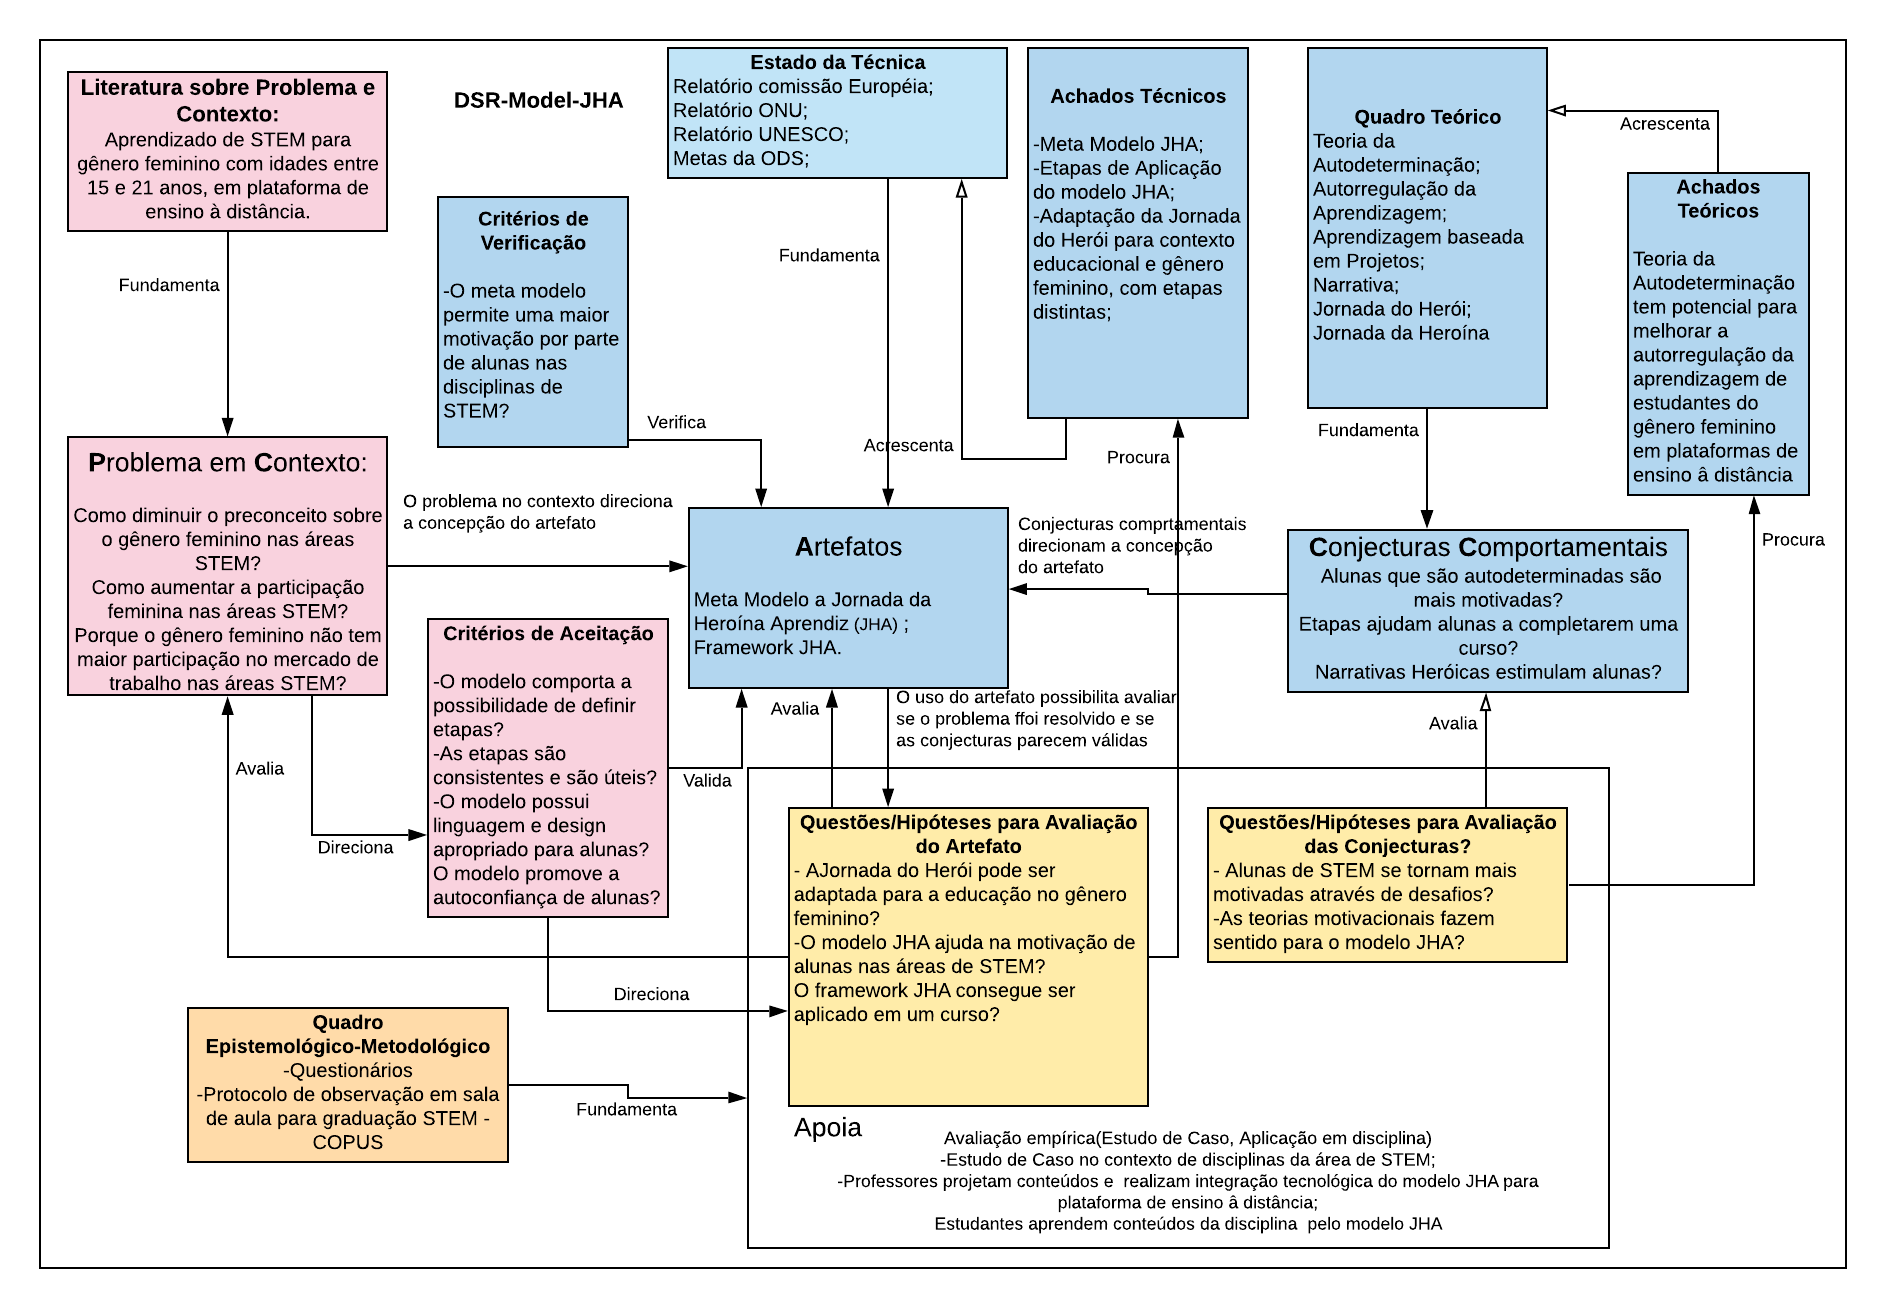
\includegraphics[width=.9\textwidth]{chaps/Images/DSRV2.png}
    \caption{Design Science Research}
    \label{fig:dsr}
\end{figure}

Uma das questões de pesquisa que importa para este estudo é: Como motivar estudantes do gênero feminino a aprenderem a se orientar por uma aprendizagem investigativa e autorregulada, utilizando recursos tecnológicos e superando desafios de forma planejada?

Literatura sobre Problema e Contexto:
Aprendizado de STEM para gênero feminino com idades entre 15 e 21 anos, em plataforma de ensino à distância.

Problema em Contexto:

Como diminuir o preconceito sobre o gênero feminino nas áreas STEM?
Como aumentar a participação feminina nas áreas STEM?
Porque o gênero feminino não tem maior participação no mercado de trabalho nas áreas STEM?

Critérios de Aceitação

-O modelo comporta a possibilidade de definir etapas?
-As etapas são consistentes e são úteis?
-O modelo possui linguagem e design apropriado para alunas? 
O modelo promove a autoconfiança de alunas?

Critérios de Verificação

-O meta modelo permite uma maior motivação por parte de alunas nas disciplinas de STEM?

Estado da Técnica
Relatório comissão Européia;
Relatório ONU;
Relatório UNESCO; 
Metas da ODS;

Achados Técnicos

-Meta Modelo JHA;
-Etapas de Aplicação do modelo JHA;
-Adaptação da Jornada do Herói para contexto educacional e gênero feminino, com etapas distintas;


Quadro Teórico
Teoria da Autodeterminação;
Autorregulação da Aprendizagem;
Aprendizagem baseada em Projetos;
Narrativa;
Jornada do Herói;
Jornada da Heroína

Achados Teóricos

Teoria da Autodeterminação tem potencial para melhorar a autorregulação da aprendizagem de estudantes do gênero feminino em plataformas de ensino â distância

Conjecturas Comportamentais
 Alunas que são autodeterminadas são mais motivadas?
Etapas ajudam alunas a completarem uma curso?
Narrativas Heróicas estimulam alunas?  

Artefatos 

Meta Modelo a Jornada da Heroína Aprendiz (JHA) ;
Framework JHA.

Quadro Epistemológico-Metodológico
-Questionários
-Protocolo de observação em sala de aula para graduação STEM - COPUS

Questões/Hipóteses para Avaliação do Artefato
- AJornada do Herói pode ser adaptada para a educação no gênero feminino?
-O modelo JHA ajuda na motivação de alunas nas áreas de STEM?
O framework JHA consegue ser aplicado em um curso?


Questões/Hipóteses para Avaliação das Conjecturas?
- Alunas de STEM se tornam mais motivadas através de desafios?
-As teorias motivacionais fazem sentido para o modelo JHA?

\section{Estrutura do documento de Tese}




